\chapter{\label{chap:intro}Análise e Discussão}
 




\section{Resultados da \textit{Survey}}

Após a conclusão do processo de coleta dados, com o objetivo de entender quais são as preocupações de desenvolvedores de software móveis no desenvolvimento de aplicações, destaca-se nessa seção o resultado obtido na survey. A survey teve um total de 20 respondentes.

O público que respondeu essa pesquisa tem em média 5 anos de experiência com desenvolvimento de aplicações  para dispositivos móveis. Em sua maioria tem experiência com a plataforma Android e desenvolve aplicativos de uso empresarial com desenvolvimento realizado em equipe.
%falar das oturas pçataformas e dos aplicativos desenvolvidos
95{\%} dos participantes da pesquisa concordam que a figura \ref{fig:1.1} que diz respeito a preocupação com o controle de acesso em sistemas desenvolvidos é importante, sendo que 75{\%} afirma que a questão é extremamente importante. Com esse resultado fica claro que existe uma preocupação dos desenvolvedores mobile com o controle de acesso de usuários. 




20{\%} dos participantes da pesquisa não e preocupam em proteger o sistemas contra tentativas forçadas e 35{\%} não soube opinar.  




\begin{figure}[t]
\centering

\paragraph{
Os respondentes foram questionados sobre sua preocupação com o controle de acesso de usuários nos sistemas que desenvolvem. Os resultados são apresentados na figura \ref{fig:1.1}
}
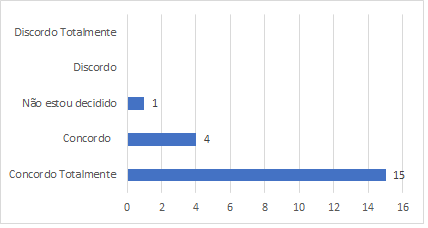
\includegraphics[scale=0.8]{figuras das questoes/1.1.PNG}
\caption{Respostas questão 1.1}

\paragraph{
Noventa e cinco por cento (95{\%}) dos respondentes (\ref{fig:1.1}) concordam que o controle de acesso em sistemas desenvolvidos é importante, considerando tanto aqueles que concordam totalmente (85{\%}) quanto aqueles que consideram a questão importante (10{\%}). Com esse resultado fica claro que existe uma preocupação dos desenvolvedores mobile com o controle de acesso de usuários.
}

\label{fig:1.1}
\end{figure}
%aqui acaba um figura
%--------------------------%
%aqui começa uma figura
\begin{figure}[!t]
\centering
\paragraph{Os respondentes foram questionados sobre sua preocupação em criar ou utilizar funcionalidades que permitam a remoção ou bloqueio de usuários no sistema. Os resultados são apresentados na figura \ref{fig:1.2}.}
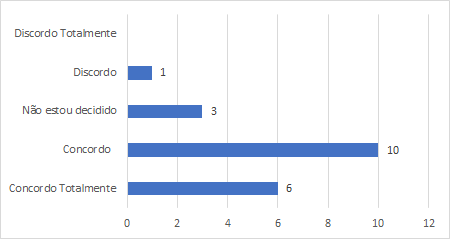
\includegraphics[scale=0.8]{figuras das questoes/1.2.PNG}
\caption{Respostas questão 1.2}

\paragraph{
Oitenta por cento (80{\%}) dos respondentes \ref{fig:1.2} concordam que criar funcionalidades que permitam remoção, bloqueio, ou desabilitação de usuários é importante, considerando tanto aqueles que concordam totalmente (30{\%}) quanto aqueles que consideram a questão apenas importante (50{\%}). Com o resultado fica claro que existe uma preocupação dos desenvolvedores com a criação destas funcionalidades.
}
\label{fig:1.2}
\end{figure}
%aqui acaba um figura
%--------------------------%
%aqui começa uma figura
\begin{figure}[!t]
\centering

\paragraph{
Os respondentes foram questionados sobre sua preocupação em desenvolver funções que permitem alteração de permissão no sistema para todos os usuários, para que seja possível fazer um gerenciamento de usuários. Os resultados são apresentados na figura \ref{fig:1.3}.
}
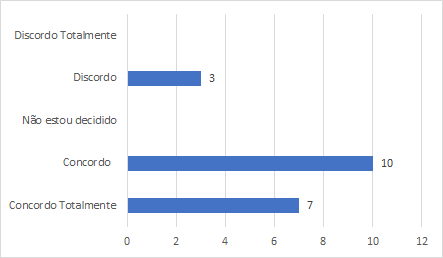
\includegraphics[scale=0.7]{figuras das questoes/1.3.png}
\caption{Respostas questão 1.3}

\paragraph{ 
Oitenta e cinco por cento (85{\%}) dos participantes afirmam se preocupar em desenvolver funcionalidades para a alteração de permissão de usuários no sistema, considerando tanto aqueles que concordam totalmente (35{\%}), quanto aqueles que consideram a questão apenas importante (50{\%}). Com esse resultado fica claro a preocupação dos desenvolvedores com a criação de tais funcionalidades. 
}

\label{fig:1.3}
\end{figure}
%aqui acaba uma figura
%--------------------------%
%aqui começa uma figura
\begin{figure}[!t]
\centering
\paragraph{
Os participantes foram questionados sobre a preocupação em criar um registro central de direitos de acesso para cada usuário. Os resultados podem ser vistos na figura \ref{fig:1.4}.
}
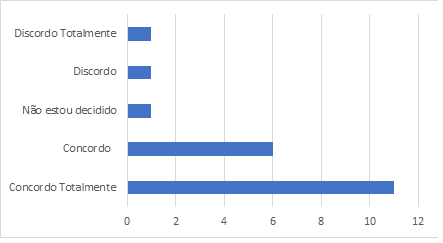
\includegraphics[scale=0.7]{figuras das questoes/1.4.png}
\caption{Respostas questão 1.4}

\paragraph{
Oitenta e cinco por cento (85{\%}) dos participantes se preocupam em criar um registro central de direitos de acesso para cada usuário, considerando tanto aqueles que concordam totalmente (55{\%}), quando aqueles que consideram apenas importante (30{\%}). Com esse resultado é possível afirmar que existe uma preocupação dos desenvolvedores com um registro central de direitos de acesso dos usuários.
}

\label{fig:1.4}
\end{figure}
%aqui acaba uma figura
%--------------------------%
%aqui começa uma figura
\begin{figure}[!t]
\centering
\paragraph{Os participantes foram questionados sobre sua preocupação em desenvolver funcionalidades que verifiquem a identidade de usuário antes de fornecer uma informação de autenticação secreta. Os resultados são apresentados na figura \ref{fig:2.1}.
}
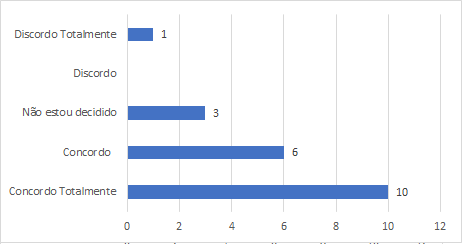
\includegraphics[scale=0.7]{figuras das questoes/2.1.png}
\caption{Respostas questão 2.1}
\paragraph{
Oitenta por cento (80{\%}) dos participantes se preocupam em desenvolver funcionalidades que verifiquem a identidade de um usuário antes de fornecer informação de autenticação secreta, considerando tanto aqueles que concordam totalmente (50{\%}) , quanto aqueles que apenas concordam (30{\%}) com a questão. Com esse resultado é possível afirmar que os desenvolvedores se preocupam com a criação de funcionalidades que verifiquem a identidade do usuário.
}
\label{fig:2.1}
\end{figure}
%aqui acaba uma figura
%--------------------------%
%aqui começa uma figura
\begin{figure}[!t]
\centering
\paragraph{
Os participantes foram questionados sobre sua preocupação a respeito do aprimoramento de funcionalidades de autenticação secreta para acessos em sistemas. Os resultados podem ser consultados na figura \ref{fig:2.2}.
}
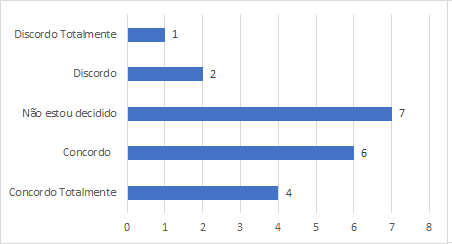
\includegraphics[scale=0.7]{figuras das questoes/2.2.png}
\caption{Respostas questão 2.2}

\paragraph{
Cinquenta por cento (50{\%}) dos participantes se preocupam em aprimorar funcionalidades de autenticação secreta em acessos nos sistemas que desenvolvem, entretanto 35{\%} não foi capaz de emitir uma opinião a respeito da pergunta e 15{\%} discorda de ser uma preocupação necessária.\todo[inline]{ Com esse resultado não é capaz de afirmar se existe uma preocupação dos desenvolvedores pois grande parte do grupo não foi capaz de emitir uma opinião a respeito do tema}
}

\label{fig:2.2}
\end{figure}
%aqui acaba uma figura
%--------------------------%
%aqui começa uma figura
\begin{figure}[!t]
\centering

\paragraph{
Os participantes foram questionados sobre a preocupação de manter a informação de autenticação secreta temporária e única pra cada pessoa. Os resultados podem ser consultados na figura \ref{fig:2.3}
}

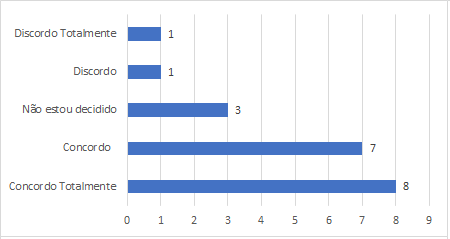
\includegraphics[scale=0.7]{figuras das questoes/2.3.png}
\caption{Respostas questão 2.3}

\paragraph{
Setenta e cinco por cento (75{\%}) dos participantes se preocupam em manter a informação de autenticação secreta única e temporária para cada pessoa, considerando tanto aqueles que concordam totalmente (40{\%}), quanto aqueles que apenas concordam (35{\%}). Com o resultado fica claro que existe uma preocupação dos desenvolvedores com o cuidado da autenticação secreta.
}

\label{fig:2.3}
\end{figure}
%aqui acaba uma figura
%--------------------------%
%aqui começa uma figura
\begin{figure}[!t]
\centering
\paragraph{
Os participantes foram questionados sobre a preocupação em fornecer recursos para que o usuário reguarde sua privacidade durante o processo de autenticação. Os resultados podem ser consultados na figura \ref{fig:2.4}
}

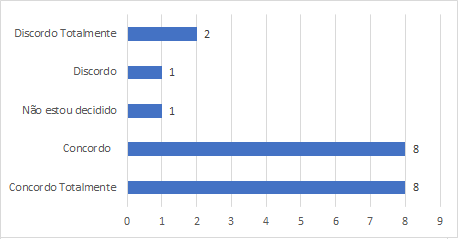
\includegraphics[scale=0.7]{figuras das questoes/2.4.png}
\caption{Respostas questão 2.4}

\paragraph{
Oitenta por cento (80{\%}) dos participantes se preocupam em fornecer recursos que possibilitem ao usuário resguardar sua privacidade durante o processo de autenticação, considerando tanto aqueles que concordam totalmente (40{\%}), quanto aqueles que apenas concordam (40{\%}). Com o resultado fica claro que existe uma preocupação dos desenvolvedores em fornecer recursos que resguardem a privacidade do usuário.
}

\label{fig:2.4}
\end{figure}
%aqui acaba uma figura
%--------------------------%
%aqui começa uma figura
\begin{figure}[!t]
\centering

\paragraph{
Os participantes foram questionados sobre a preocupação de não mostrar dados sensíveis de usuários até o processo de Log-on. Os resultados podem ser consultados na figura \ref{fig:2.5}
}

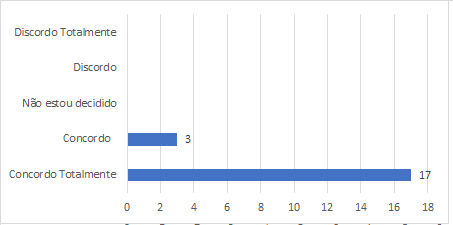
\includegraphics[scale=0.7]{figuras das questoes/2.5.png}
\caption{Respostas questão 2.5}

\paragraph{
Cem por cento (100{\%}) dos participantes se preocupam em não mostrar dados sensíveis dos usuários durante o processo de Log-on. Com o resultado é possível ver a unanimidade na importância que os desenvolvedores dão a essa questão.
}
\label{fig:2.5}
\end{figure}
%aqui acaba uma figura
%--------------------------%
%aqui começa uma figura
\begin{figure}[!t]
\centering
\paragraph{
Os participantes foram questionados sobre a preocupação de validar as informação de entrada no sistema somante quando os dados estiverem completos.Os resultados podem ser consultados na figura \ref{fig:2.6}
}
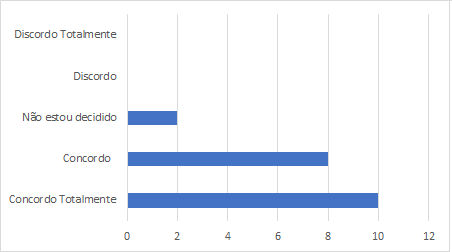
\includegraphics[scale=0.7]{figuras das questoes/2.6.png}
\caption{Respostas questão 2.6}

\paragraph{
Noventa por cento (90{\%}) dos participantes se preocupam em validar os dados de entrada no sistema somente quando estiverem completos, considerando tanto aqueles que concordam totalmente (50{\%}), quanto aqueles que apenas concordam (40{\%}). Com esse resultado fica claro que existe uma preocupação dos desenvolvedores em validar os dados do usuário somente quando estiverem totalmente completos.
}
\label{fig:2.6}
\end{figure}
%aqui acaba uma figura
%--------------------------%
%aqui começa uma figura
\begin{figure}[!t]
\centering

\paragraph{
Os participante foram questionados sobre a preocupação de não revelar qual parte do dado esta correto ou incorreto durante um processo de entrada no sistema. Os resultados podem ser consultados na figura \ref{fig:2.7}
} 

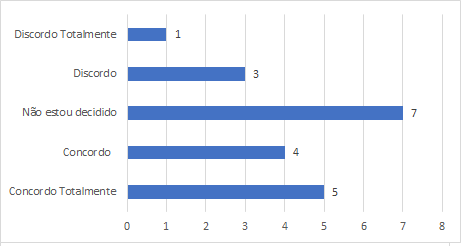
\includegraphics[scale=0.7]{figuras das questoes/2.7.png}
\caption{Respostas questão 2.7}
\todo[inline]{trocar o gráfico ele esta errado}
\paragraph{
Oitenta e cinco por cento (85{\%}) dos participantes se preocupam em não revelar qual parte do dado esta correto ou incorreto em um processo de entrada no sistema, considerando tanto aqueles que concordam totalmente (65{\%}), quanto aqueles que apenas concordam (20{\%}). Com esse resultado fica claro a preocupação do desenvolvedores em não fornecer ajuda a um usuário possivelmente mal intencionado.
}
\label{fig:2.7}
\end{figure}
%aqui acaba uma figura
%--------------------------%
%aqui começa uma figura
\begin{figure}[!t]
\centering

\paragraph{Os participantes foram questionados sobre a preocupação de proteger o sistema contra tentativas consecutivas de entrada forçada no sistema. Os resultados podem ser consultados na figura \ref{fig:2.8}.
}

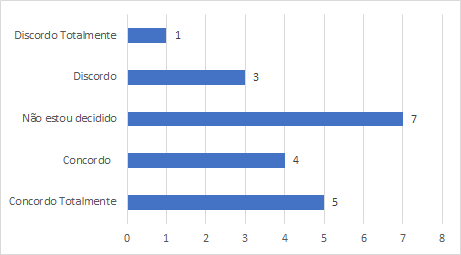
\includegraphics[scale=0.7]{figuras das questoes/2.8.png}
\caption{Respostas questão 2.8}

\paragraph{
Quarenta e cinco por cento (45{\%}) dos participantes se preocupam em proteger o sistema contra tentativas consecutiva de entrada forçada no sistema, contudo 35{\%} dos respondentes não foi capaz de opinar sobre a questão e 20{\%} discorda que seja um preocupação.Com esse resultado não é possível afirmar se existe uma preocupação dos desenvolvedores com proteção do sistema contra um tentativa forçada de entrada no sistema.
}

\label{fig:2.8}
\end{figure}
%aqui acaba uma figura
%--------------------------%
%aqui começa uma figura
\begin{figure}[!t]
\centering
\paragraph{Os participantes foram questionados sobre a preocupação de comunicar um evento de segurança caso uma tentativa ou violação bem sucedida de entrada no sistema seja realizada. Os resultados podem ser consultados na figura \ref{fig:2.9}.}
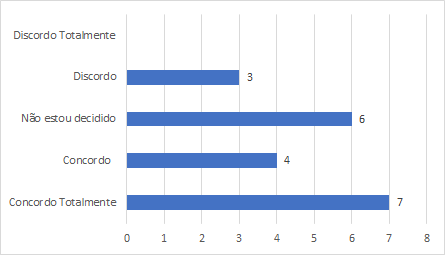
\includegraphics[scale=0.7]{figuras das questoes/2.9.png}
\caption{Respostas questão 2.9}

\paragraph{Cinquenta e cinco por cento (55{\%}) dos participantes se preocupam em comunicar eventos de segurança, contudo 30{\%} não souberam responder e 15{\%} discordaram. Com esse resultado é possível afirmar que existe uma preocupação dos desenvolvedores sobra a comunicação de eventos de segurança.} 

\label{fig:2.9}
\end{figure}
%aqui acaba uma figura
%--------------------------%
%aqui começa uma figura
\begin{figure}[!t]
\centering
\paragraph{Os participante foram questionados sobre a preocupação encerrar sessões após um período de inatividade. Os resultados podem ser consultados na figura \ref{fig:2.10}.}

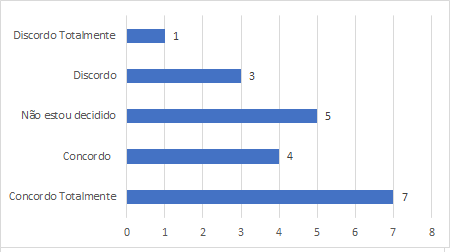
\includegraphics[scale=0.7]{figuras das questoes/2.10.png}
\caption{Respostas questão 2.10}

\paragraph{Cinquenta e cinco por cento (55{\%}) dos participantes se preocupam em encerrar sessões inativas após um período de inatividade, contudo 25{\%} não soube opinar e 20{\%} discordaram que seria uma preocupação. Com esse resultado é possível  ver que existe uma preocupação dos desenvolvedores quanto ao tempo de inatividade.
}
\label{fig:2.10}
\end{figure}

%aqui acaba uma figura
%--------------------------%
%aqui começa uma figura

\begin{figure}[!t]
\centering
\paragraph{Os participantes foram questionados sobre a preocupação em criar sistemas que obriguem a escolha de uma senha de qualidade por parte do usuário. Os resultados podem ser consultados na figura \ref{fig:2.11}. }

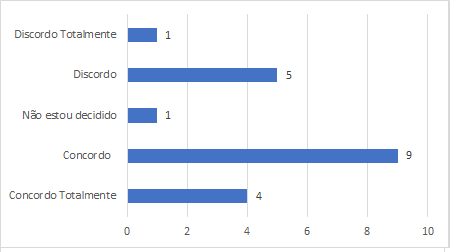
\includegraphics[scale=0.7]{figuras das questoes/2.11.png}
\caption{Respostas questão 2.11}

\paragraph{
sessenta e cinco por cento (65{\%}) dos participantes se preocupa em obrigar o usuário a criar um senha de qualidade, entretanto 30{\%} descorda que  isso seja uma preocupação. Com o resultado é possível afirmar que existe uma preocupação dos desenvolvedores em obrigar o usuário criar senhas de qualidade, \todo[inline]{entretanto seria relevante entender o motivo que levou os 30{\%} dos participantes a discordarem da importância.} 
}

\label{fig:2.11}
\end{figure}

%aqui acaba uma figura
%--------------------------%
%aqui começa uma figura

\begin{figure}[!t]
\centering
\paragraph{Os participantes foram questionados sobre a preocupação em desenvolver sistemas que obriguem o usuário a mudar as suas senhas temporárias no primeiro acesso ao sistema. Os resultados podem ser consultados na figura \ref{fig:2.12}. }
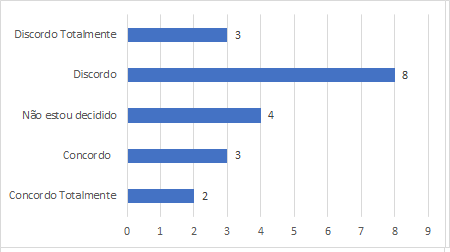
\includegraphics[scale=0.7]{figuras das questoes/2.12.png}
\caption{Respostas questão 2.12}
\paragraph{
Cinquenta e cinto por cento (55{\%}) dos respondentes dos participantes não se preocupam em obrigar o usuário a trocar a senha temporária de primeiro acesso, 20{\%} não soube responder e Apenas 25{\%} dos participantes concordaram que obrigar a troca de senha seria uma preocupação. \todo[inline]{Com esse resultado é possível concluir que não existe uma preocupação forte dos desenvolvedores sobre essa questão.}
}

\label{fig:2.12}
\end{figure}

%aqui acaba uma figura
%--------------------------%
%aqui começa uma figura

\begin{figure}[!t]
\centering
\paragraph{Os participantes foram questionados sobre a preocupação de não permitir que a senha possa ser mostrada na tela quando digitada ( foi usado o "olho" como exemplo ). Os resultados podem ser consultados na figura \ref{fig:2.13}. 
}
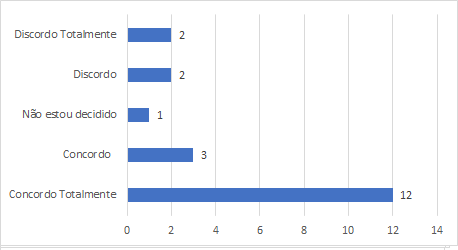
\includegraphics[scale=0.7]{figuras das questoes/2.13.png}
\caption{Respostas questão 2.13}

\paragraph{
Setenta e cinco por cento (75{\%}) dos respondentes se preocupam em resguardar a visualização da senha quando digitada.  Com esse resultado é possível  ver que existe uma preocupação dos desenvolvedores quanto a proteção da visualização da senha.
}

\label{fig:2.13}
\end{figure}
%aqui acaba uma figura
%--------------------------%
%aqui começa uma figura
\begin{figure}[!t]
\centering

\paragraph{Os respondentes foram questionados sobre a preocupação com o uso de criptografia para a proteção das informações sensíveis durante a comunicação em dispositivos móveis.  Os resultados podem ser consultados na figura \ref{fig:3.1}.
}
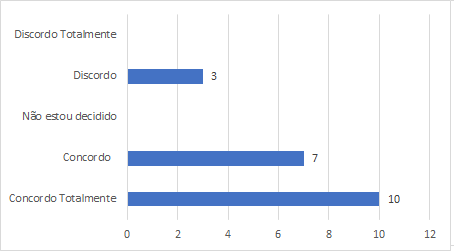
\includegraphics[scale=0.7]{figuras das questoes/3.1.png}
\caption{Respostas questão 3.1}

\paragraph{Oitenta e cinco por cento (85{\%}) dos participantes se preocupam usar criptografia para a proteção de informações, considerando tanto aqueles que concordam totalmente (50{\%}), quanto aqueles que apenas concordam (35{\%}). Com o resultado fica claro que existe uma preocupação dos desenvolvedores com a utilização de criptografia.
}

\label{fig:3.1}
\end{figure}
%aqui acaba uma figura
%--------------------------%
%aqui começa uma figura
\begin{figure}[!t]
\centering
\paragraph{
Os participantes foram questionados sobre a preocupação em gerar chaves para diferentes sistemas sistemas criptográficos e diferentes aplicações. s resultados podem ser consultados na figura \ref{fig:3.2}.}
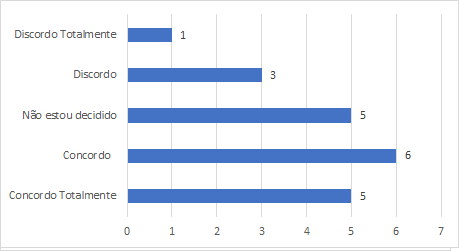
\includegraphics[scale=0.7]{figuras das questoes/3.2.png}
\caption{Respostas questão 3.2}

\paragraph{
Cinquenta e cinco por cento (55{\%}) dos participantes se preocupam em gerar chaves para diferentes sistemas criptográfico, 25{\%} não souberam opinar e 20{\%} discordam que seja uma preocupação. Com esse resultado é possível ver que a maioria dos desenvolvedores considera que gerar diferentes chaves criptográficas é importante.
}

\label{fig:3.2}
\end{figure}
%aqui acaba uma figura
%--------------------------%
%aqui começa uma figura
\begin{figure}[!t]
\centering

\paragraph{Os participantes foram questionados sobre a preocupação com os impactos da segurança da informação quando ocorre alguma mudança no sistema. Os resultados podem ser consultados na figura \ref{fig:4.1}.}
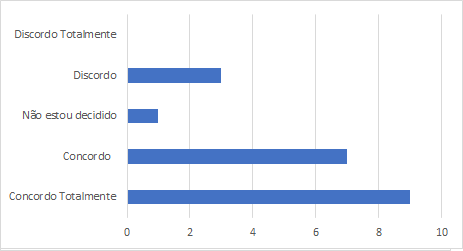
\includegraphics[scale=0.7]{figuras das questoes/4.1.png}
\caption{Respostas questão 4.1}
\paragraph{Oitenta por cento (85{\%}) do participantes se preocupam com os impactos da segurança da informação quando ocorre alguma mudança no sistema, considerando tanto aqueles que concordam totalmente (45{\%}), quanto aqueles que apenas concordam (35{\%}).Com esse resultado fica claro que existe uma preocupação dos desenvolvedores.}

\label{fig:4.1}
\end{figure}
%aqui acaba uma figura
%--------------------------%
%aqui começa uma figura
\begin{figure}[!t]
\centering
\paragraph{Os participantes foram questionados sobre a preocupação de  criar mecanismos para atender o crescimento da aplicação e possibilitar suportar demanda variável de acessos. Os resultados podem ser consultados na figura \ref{fig:4.2}.}

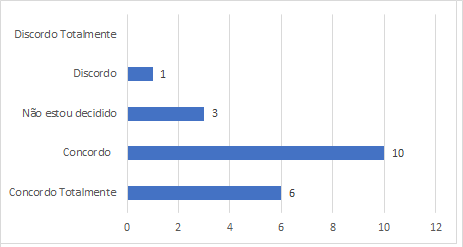
\includegraphics[scale=0.7]{figuras das questoes/4.2.png}
\caption{Respostas questão 4.2}
\paragraph{Oitenta por cento (80{\%}) dos participantes se preocupam em criar mecanismos para atender o crescimento da aplicação, considerando tanto aqueles que concordam totalmente (30{\%}), quanto aqueles que apenas concordam (50{\%}).Com esse resultado fica claro que existe uma preocupação dos desenvolvedores.}
\label{fig:4.2}
\end{figure}
%aqui acaba uma figura
%--------------------------%
%aqui começa uma figura
\begin{figure}[!t]
\centering
\paragraph{Os participantes foram questionados sobre a preocupação de não copiar dados sensíveis para o ambiente de teste. s resultados podem ser consultados na figura \ref{fig:4.3}.}

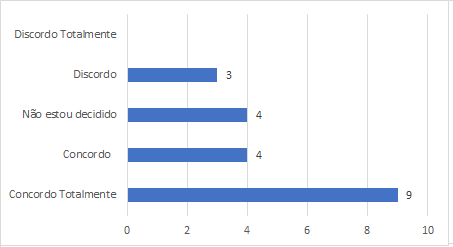
\includegraphics[scale=0.7]{figuras das questoes/4.3.png}
\caption{Respostas questão 4.3}
\paragraph{sessenta e cinco por cento (65{\%}) dos participantes se preocupam em não copiar dados sensíveis para o ambiante de teste, considerando tanto aqueles que concordam totalmente (45{\%}), quanto aqueles que apenas concordam (20{\%}).Com esse resultado fica claro que existe uma preocupação dos desenvolvedores em não copiar dados sensíveis para o ambiente de teste} 

\label{fig:4.3}
\end{figure}
%aqui acaba uma figura
%--------------------------%
%aqui começa uma figura
\begin{figure}[!t]
\centering
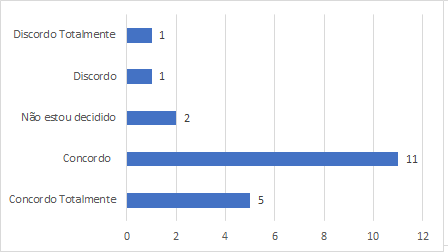
\includegraphics[scale=0.7]{figuras das questoes/5.1.png}
\caption{Respostas questão 5.1}
\end{figure}

\begin{figure}[!t]
\centering
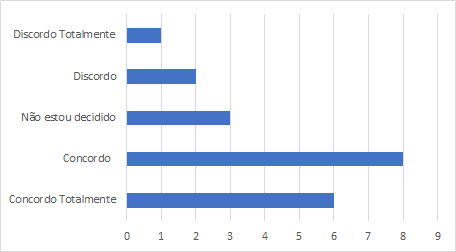
\includegraphics[scale=0.7]{figuras das questoes/5.2.png}
\caption{Respostas questão 5.2}
\end{figure}

\begin{figure}[!t]
\centering
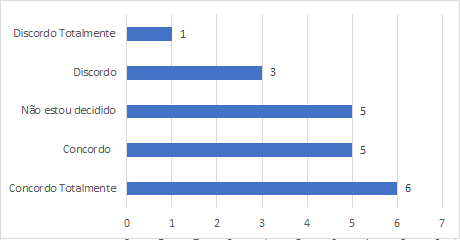
\includegraphics[scale=0.7]{figuras das questoes/5.3.png}
\caption{Respostas questão 5.3}
\end{figure}

\begin{figure}[!t]
\centering
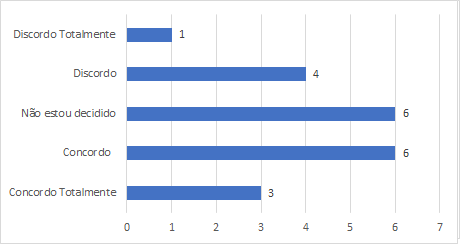
\includegraphics[scale=0.7]{figuras das questoes/5.4.png}
\caption{Respostas questão 5.4}
\end{figure}
 
\begin{figure}[!t]
\centering
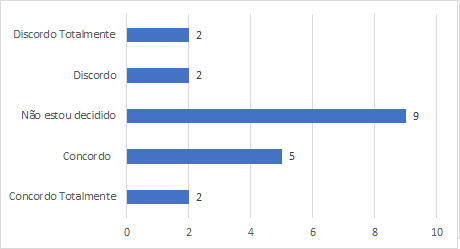
\includegraphics[scale=0.7]{figuras das questoes/5.5.png}
\caption{Respostas questão 5.5}
\end{figure}
 
\begin{figure}[!t]
\centering
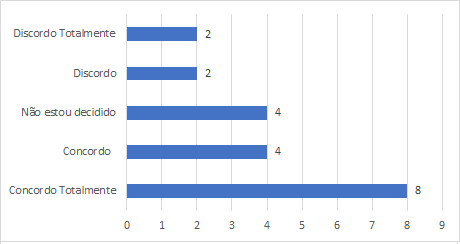
\includegraphics[scale=0.7]{figuras das questoes/5.6.png}
\caption{Respostas questão 5.6}
\end{figure}
   
\begin{figure}[!t]
\centering
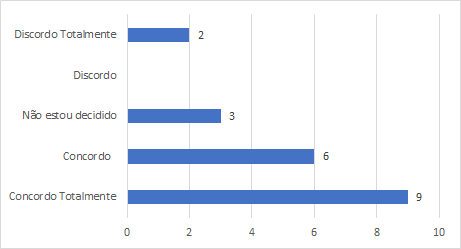
\includegraphics[scale=0.7]{figuras das questoes/6.1.png}
\caption{Respostas questão 6.1}
\end{figure}

\begin{figure}[!t]
\centering
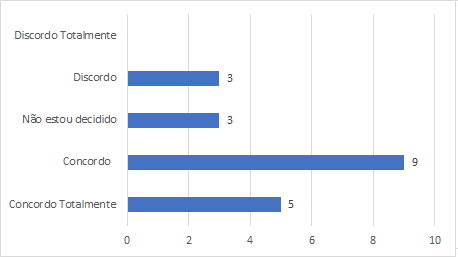
\includegraphics[scale=0.7]{figuras das questoes/6.2.png}
\caption{Respostas questão 6.2}
\end{figure}

\begin{figure}[!t]
\centering
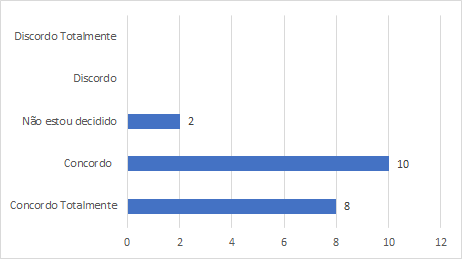
\includegraphics[scale=0.7]{figuras das questoes/6.3.png}
\caption{Respostas questão 6.3}
\end{figure}

\begin{figure}[!t]
\centering
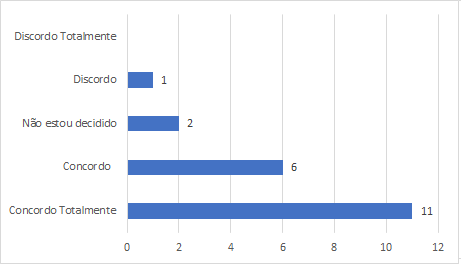
\includegraphics[scale=0.7]{figuras das questoes/6.4.png}
\caption{Respostas questão 6.4}
\end{figure}

\begin{figure}[!t]
\centering
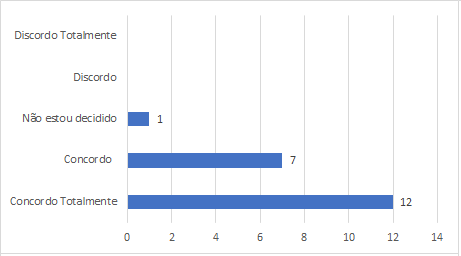
\includegraphics[scale=0.7]{figuras das questoes/6.5.png}
\caption{Respostas questão 6.5}
\end{figure}

\begin{figure}[!t]
\centering
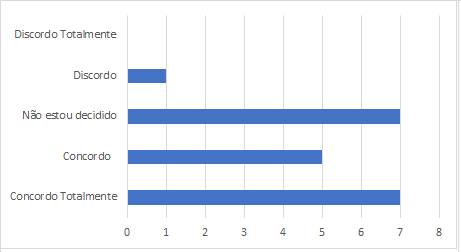
\includegraphics[scale=0.7]{figuras das questoes/6.6.png}
\caption{Respostas questão 6.6}
\end{figure}

\begin{figure}[!t]
\centering
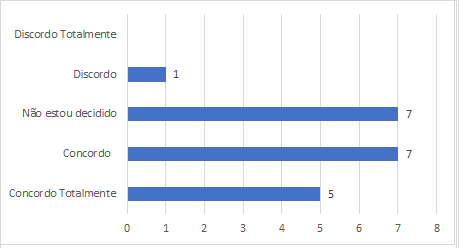
\includegraphics[scale=0.7]{figuras das questoes/6.7.png}
\caption{Respostas questão 6.7}
\end{figure}

\begin{figure}[!t]
\centering
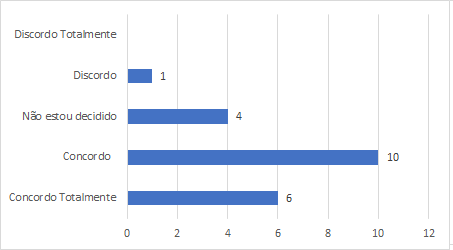
\includegraphics[scale=0.7]{figuras das questoes/6.8.png}
\caption{Respostas questão 6.8}
\end{figure}

\begin{figure}[!t]
\centering
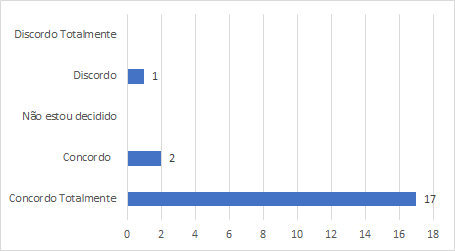
\includegraphics[scale=0.7]{figuras das questoes/6.9.png}
\caption{Respostas questão 6.9}
\end{figure}

\begin{figure}[!t]
\centering
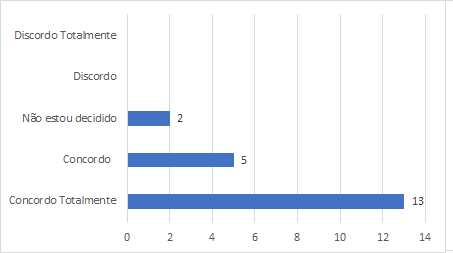
\includegraphics[scale=0.7]{figuras das questoes/6.10.png}
\caption{Respostas questão 6.11}
\end{figure}

\begin{figure}[!t]
\centering
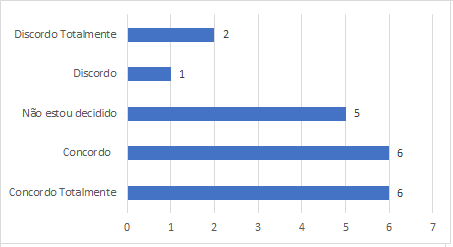
\includegraphics[scale=0.7]{figuras das questoes/6.11.png}
\caption{Respostas questão 6.11}
\end{figure}

\begin{figure}[!t]
\centering
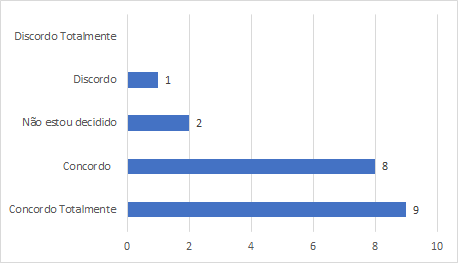
\includegraphics[scale=0.7]{figuras das questoes/6.12.png}
\caption{Respostas questão 6.12}
\end{figure}

\begin{figure}[!t]
\centering
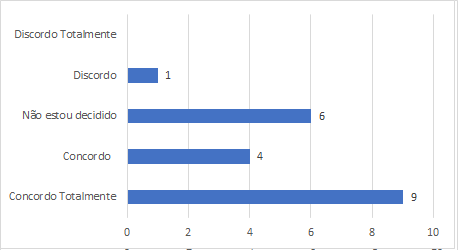
\includegraphics[scale=0.7]{figuras das questoes/6.13.png}
\caption{Respostas questão 6.13}
\end{figure}

\begin{figure}[!t]
\centering
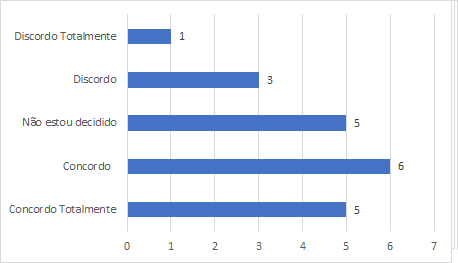
\includegraphics[scale=0.7]{figuras das questoes/6.14.png}
\caption{Respostas questão 6.14}
\end{figure}

\begin{figure}[!t]
\centering
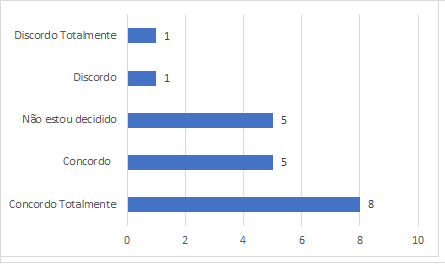
\includegraphics[scale=0.7]{figuras das questoes/6.15.png}
\caption{Respostas questão 6.15}
\end{figure}

\begin{figure}[!t]
\centering
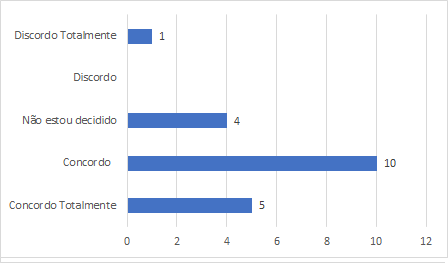
\includegraphics[scale=0.7]{figuras das questoes/6.16.png}
\caption{Respostas questão 6.16}
\end{figure}

\begin{figure}[t]
\centering
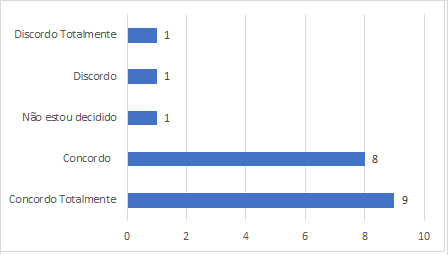
\includegraphics[scale=0.7]{figuras das questoes/6.17.png}
\caption{Respostas questão 6.17}
\end{figure}

\begin{itemize}
%\item Especialista 2: Confirmou-se com o especialista que será realizada a entrevista para examinar a qualidade das perguntas elaboradas com o especialista 1.
\end{itemize}


 

 

 
